\begin{figure}[htbp]
    \centering
    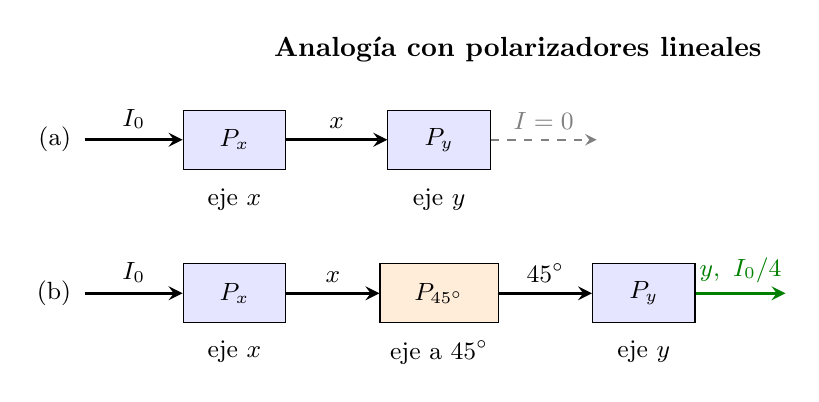
\begin{tikzpicture}[>=stealth, every node/.style={font=\small}]
        \node[font=\bfseries] at (5.0,2.0) {Analogía con polarizadores lineales};

        \node[draw,fill=blue!10,minimum width=1.3cm,minimum height=0.75cm] (x1) at (1.4,0.85) {$P_x$};
        \node[draw,fill=blue!10,minimum width=1.3cm,minimum height=0.75cm] (y1) at (4.0,0.85) {$P_y$};
        \draw[->,very thick] (-0.5,0.85) -- (x1.west) node[midway,above] {$I_0$};
        \draw[->,very thick] (x1.east) -- (y1.west) node[midway,above] {$x$};
        \draw[->,thick,dashed,gray] (y1.east) -- (6.0,0.85) node[midway,above] {$I=0$};
        \node[below] at (1.4,0.35) {eje $x$};
        \node[below] at (4.0,0.35) {eje $y$};
        \node[left] at (-0.55,0.85) {(a)};

        \node[draw,fill=blue!10,minimum width=1.3cm,minimum height=0.75cm] (x2) at (1.4,-1.1) {$P_x$};
        \node[draw,fill=orange!15,minimum width=1.5cm,minimum height=0.75cm] (d45) at (4.0,-1.1) {$P_{45^\circ}$};
        \node[draw,fill=blue!10,minimum width=1.3cm,minimum height=0.75cm] (y2) at (6.6,-1.1) {$P_y$};
        \draw[->,very thick] (-0.5,-1.1) -- (x2.west) node[midway,above] {$I_0$};
        \draw[->,very thick] (x2.east) -- (d45.west) node[midway,above] {$x$};
        \draw[->,very thick] (d45.east) -- (y2.west) node[midway,above] {$45^\circ$};
        \draw[->,very thick,green!50!black] (y2.east) -- (8.4,-1.1) node[midway,above] {$y,\ I_0/4$};
        \node[below] at (1.4,-1.58) {eje $x$};
        \node[below] at (4.0,-1.58) {eje a $45^\circ$};
        \node[below] at (6.6,-1.58) {eje $y$};
        \node[left] at (-0.55,-1.1) {(b)};
    \end{tikzpicture}
    \caption{Polarizadores cruzados bloquean la luz, pero un polarizador intermedio a $45^\circ$ transmite una fracción no nula ($I_0/4$) a través del último filtro.}
    \label{fig:polarizadores}
\end{figure}